\documentclass[border=1pt]{standalone}
% Shared preamble for standalone figures in this directory.
% Compile with XeLaTeX from 讲义/figs, or via the figures target.
\usepackage{ctex}
\usepackage{amsmath}
\usepackage{amssymb}
\usepackage{bm}
\usepackage{mathtools}
\usepackage{tikz}
\renewcommand{\vec}[1]{\boldsymbol{#1}}
\newcommand{\cC}{\mathcal{C}}
\newcommand{\cD}{\mathcal{D}}
\newcommand{\R}{\mathbf{R}}
\usetikzlibrary{
    arrows.meta,
    calc,
    decorations.markings,
    angles,
    quotes,
    positioning,
    patterns,
    shapes.geometric
}

\begin{document}
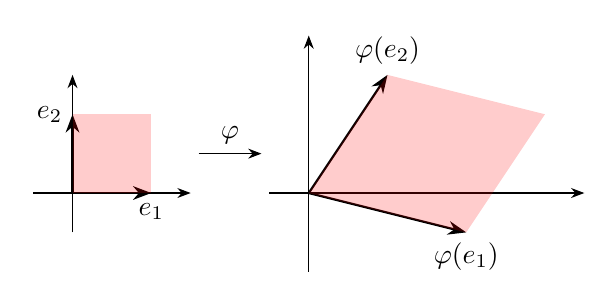
\begin{tikzpicture}[>=Stealth, scale=1]
    \draw[->] (-0.5, 0) -- (1.5, 0);
    \draw[->] (0, -0.5) -- (0, 1.5);
    \draw[thick, ->] (0, 0) -- (1, 0) node[below]{$e_1$};
    \draw[thick, ->] (0, 0) -- (0, 1) node[left]{$e_2$};
    \fill[red, opacity=0.2] (0, 0) -- (1, 0) -- (1, 1) -- (0, 1);
    \begin{scope}[shift={(3, 0)}]
        \draw[->] (-.5, 0) -- (3.5, 0);
        \draw[->] (0, -1) -- (0, 2);
        \draw[thick, ->] (0, 0) -- (2, -.5)
            node[below]{$\varphi(e_1)$};
        \draw[thick, ->] (0, 0) -- (1, 1.5)
            node[above]{$\varphi(e_2)$};
        \fill[red, opacity=0.2] (0, 0) -- (2, -.5)
            -- (3, 1) -- (1, 1.5);
    \end{scope}
    \draw[->] (1.6, 0.5) -- node[above]{$\varphi$}
         (2.4, 0.5);
\end{tikzpicture}

\end{document}
